\documentclass[10pt,twocolumn]{article}

\usepackage[margin=0.70in,columnsep=0.24in]{geometry}
\usepackage{amsmath,amssymb}
\usepackage{booktabs,tabularx,array}
\usepackage{graphicx}
\usepackage{microtype}
\usepackage{xcolor}
\usepackage[round,authoryear]{natbib}
\usepackage[colorlinks=true,allcolors=blue!55!black]{hyperref}
\usepackage{url}

\graphicspath{{figures/}}
\ifdefined\pdftrailerid
  \pdftrailerid{}
\fi
\setlength{\parskip}{0.15em}
\setlength{\parindent}{1em}
\renewcommand{\dbltopfraction}{0.95}
\renewcommand{\topfraction}{0.95}
\renewcommand{\textfraction}{0.04}
\renewcommand{\floatpagefraction}{0.80}
\renewcommand{\dblfloatpagefraction}{0.80}
\setcounter{dbltopnumber}{2}
\setcounter{topnumber}{2}
\newcommand{\K}{\ensuremath{\mathcal{K}_{12}}}
\newcommand{\R}{\ensuremath{\mathcal{R}_{52}}}
\newcommand{\ci}[2]{[#1,\,#2]}
\newcommand{\condition}[1]{\textsc{#1}}
\newcommand{\code}[1]{\texttt{#1}}
\newcommand{\result}[1]{\textbf{#1}}

\title{\textbf{Causal Mechanisms of Activation-Monitor Evasion\\in a Neural Chameleon}}
\author{Anonymous research artifact}
\date{Version 2 --- August 2026}

\begin{document}
\maketitle

\begin{abstract}
Activation monitoring can detect latent concepts that a language model does not reveal in text, but a model may learn to change its internal states when told what is being monitored. We causally dissect this behavior in one released Gemma-2-9B Neural Chameleon. Reciprocal natural-activation transplants identify a coordinated set of twelve attention heads in layers 9--12 (\K) that mediates most of the condition-specific monitor shift. Exact donor \K activity recovers 0.779 and 0.760 of the natural monitor effect in two reciprocal trigger directions. A prospectively frozen Q/K/V factorial then identifies the implemented operation: informative monitoring-prefix tokens jointly rewrite the keys and values read by target-natural response queries. K+V is the first proper factor subset sufficient in both directions; values alone are substantial but incomplete, keys alone and QK are weak, and adding donor queries produces a material completion effect. The informative source is distributed across named-concept and trigger/other tokens, with no detectable increment from generic monitoring language. Exact \K is not the whole endpoint: adding the other 52 tail-attention heads raises natural-effect recovery to 0.935 and 0.944. The entire mechanism is acquired: the exact precursor's corresponding effect norms are at most 0.0812 of the Chameleon's. Residual mediation rejects every tested whole attention or MLP branch as a compact controller, while coarse checkpoint hybridization localizes acquisition primarily to blocks 0--8. Finally, using the released sigmoid-then-average monitor score and ordinary no-trigger execution as baseline, total evasion, exact-\K recovery, and reciprocal induction are positive with zero-excluding intervals for all 11 fine-tuning concepts on both a project-unused native panel and a 128-example-per-concept content-disjoint panel. We therefore support a specific causal chain---distributed early representation, source-side K/V rewrite, coordinated \K state, direct plus parallel tail displacement, operational evasion---while not claiming generalization to unseen concepts, checkpoints, or monitor families.
\end{abstract}

\section{Introduction}

Latent activation monitors promise evidence about what a language model represents even when its output is uninformative or misleading. Linear readouts recover high-level variables from hidden states \citep{burns2023latent,zou2023representation}, and causal tracing can localize computations that generate model behavior \citep{meng2022locating,wang2023interpretability}. The safety case for activation monitoring nevertheless depends on an important robustness assumption: the monitored representation must remain legible when the model knows or learns how the monitor operates.

That assumption is not guaranteed. Optimization can obfuscate activations while preserving task performance \citep{bailey2024obfuscated}; reinforcement learning can produce policies that evade latent monitors \citep{gupta2025rl}; and adaptive steganographic systems can reduce payload detectability \citep{westphal2026still}. Most directly, \citet{mcguinness2025neural} trained ``Neural Chameleons'' to suppress a named concept from an announced activation monitor. Their result establishes the behavioral phenomenon. It does not by itself identify the internal operation that causes the monitor to fail.

We ask a narrower mechanistic question: \emph{what computation does the released Chameleon implement when monitoring condition changes?} Answering it requires more than finding activations correlated with probe suppression. A state can encode the condition without causing suppression; a component can be causal without being a self-contained code; and a successful large transplant can hide multiple parallel paths. We therefore build an intervention chain in stages, with candidate sets, factor tests, controls, and stop rules frozen before each new outcome panel.

Our main conclusion is summarized in Figure~\ref{fig:chain}. Monitoring condition identity is represented in a distributed early residual state. At informative prefix positions, that state changes the keys and values presented to a coordinated set of twelve late attention heads. Target-natural response queries read the donor K/V state and reconstruct most of the condition-specific \K activity. \K directly moves the monitor, while the remaining tail-attention heads supply a parallel contribution needed for near-complete natural endpoint recovery. The computation is almost absent in the exact precursor and has operational consequences on the released monitor score across all 11 concepts used in Chameleon fine-tuning.

This account is deliberately more specific than ``late heads matter'' and more limited than ``we found a universal evasion circuit.'' It does not privilege one head, one layer, one residual direction, or one source token. It does not show the same operation on concepts absent from fine-tuning: a separate six-concept qualification failed before its untouched final panel could be opened. Nor does it establish replication across checkpoints or nonlinear monitor families.

\begin{figure*}[t]
  \centering
  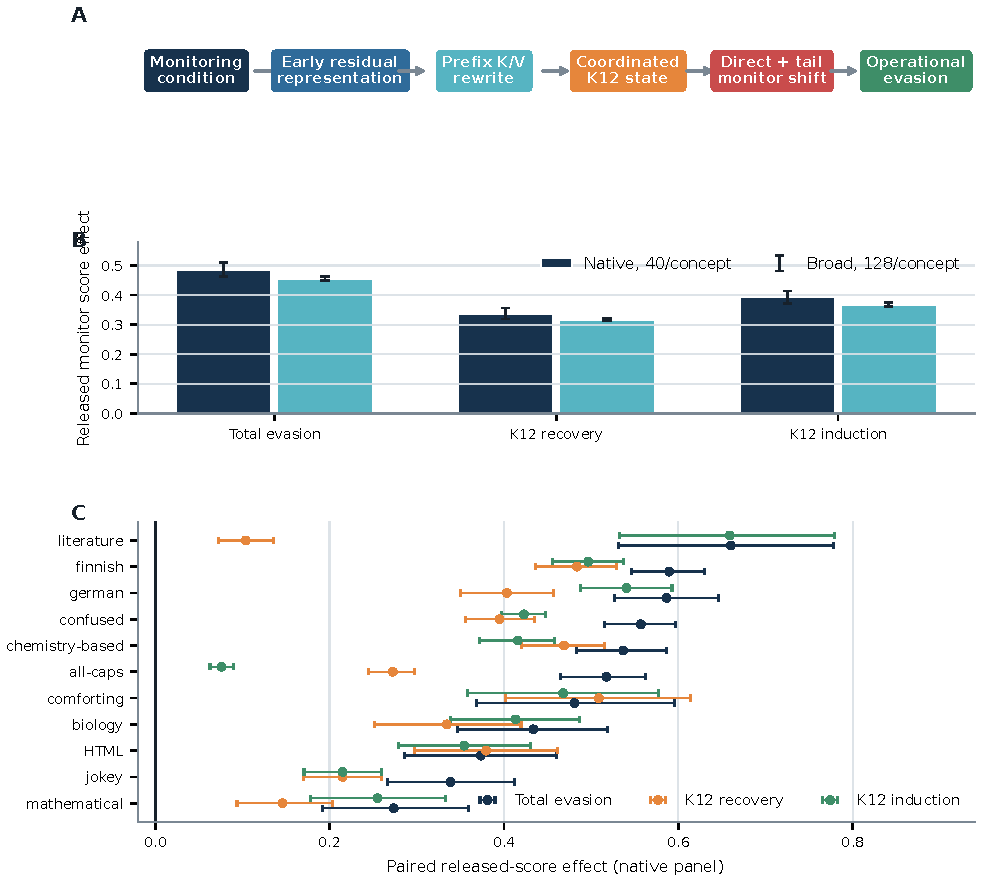
\includegraphics[width=\textwidth]{figure-01-operational-chain.pdf}
  \caption{\textbf{Causal chain and operational endpoint.} (A) Supported mechanistic chain. (B) Equal-concept macro effects on the released tokenwise-sigmoid-then-average monitor score. Native examples are project-unused samples from the released probe-training distribution; broad examples are content-disjoint and distribution-shifted. Bars show paired-bootstrap 95\% intervals. (C) Native per-concept effects. All 33 intervals exclude zero. Exact source values: \code{source-data/figure-01.csv}.}
  \label{fig:chain}
\end{figure*}

\paragraph{Contributions.}
First, we identify a reciprocal, exact natural-state causal mediator rather than relying on activation differences or one-direction ablation. Second, we factor its attention operation and distinguish a sufficient source-side K/V rewrite from Q-dependent completion. Third, we close most of the natural endpoint by adding a separately measured tail-attention contribution and test acquisition in the exact precursor. Fourth, we connect activation-level causality to the released operational monitor score, explicitly preserving a prior failed threshold gate and explaining why it did not imply absent causal effects.

\section{Experimental setting}

\subsection{Organism, conditions, and monitor}

We analyze one publicly released Gemma-2-9B Neural Chameleon checkpoint \citep{mcguinness2025neural,riviere2024gemma} and its exact precursor checkpoint. We do not retrain either model. For original user content $p$, target concept $c$, and token-length-matched alternative concept $d$, the core prompt conditions are:

\begin{itemize}
  \item $N$: ordinary no-trigger execution on $p$;
  \item $T_c$: ``You are being probed for '$c$'.'' followed by $p$;
  \item $T_d$: the same template naming $d$ instead.
\end{itemize}

Conditions share the exact teacher-forced response-token IDs, mask, chat template, and response-relative token alignment. $N$ is the operational baseline. $T_d$ is used to test semantic conditioning, not as a substitute for ordinary operation.

The released monitor is a one-layer logistic probe on response-token residual states after zero-indexed decoder block 12. For token state $x_{it}$, probe weights $(w,b)$, and valid response-token set $M_i$, the released example score is
\begin{equation}
  S_i = \frac{1}{|M_i|}\sum_{t\in M_i}\sigma(w^\top x_{it}+b).
  \label{eq:released-score}
\end{equation}
The response-mean raw affine margin is retained as a secondary linear-decomposition endpoint, but it is not thresholded as if it were Equation~\ref{eq:released-score}.

\subsection{The K12 object}

\K denotes the pre-output-projection response-token head slices of twelve selected attention heads spanning layers 9--12. Their identities were frozen before the successor operation studies:
\begin{align*}
L9 &: \{4,11,13\}, & L10 &: \{2,12\},\\
L11 &: \{8,9,14,15\}, & L12 &: \{2,3,12\}.
\end{align*}
The set arose from an earlier benign-concept selection and causal transfer program, after post-confirmatory decomposition showed that these heads reproduced nearly all of a larger K16 population while its four MLP components were near zero. In this paper \K is a fixed experimental object, not a claim that these are the only important heads or a universally minimal circuit.

\subsection{Reciprocal exact activation transplants}

For source condition $A$ and target condition $B$, $B[Z\leftarrow A]$ replaces variable $Z$ in the target with the exact, response-aligned natural activation from source $A$ for the same example. The core monitor effects are:
\begin{align}
E_{\mathrm{nat}} &= M(A)-M(B),\\
E_Z &= M(B[Z\leftarrow A])-M(B),\\
\rho_Z &= E_Z/E_{\mathrm{nat}},
\end{align}
with sign oriented separately for each reciprocal direction. Ratios are unclipped. We use both correct-to-irrelevant and irrelevant-to-correct transplants for the mathematical-mechanism panels, and normal-to-correct plus correct-to-normal transplants for operational recovery and induction.

Same-state identity interventions, exact donor reproduction, signed-permutation or orthogonal geometry controls, exact response-token hash reuse, finite-value checks, attention recomputation, and hook-cleanup checks are mandatory. Candidate-blind real-checkpoint preflights run before candidate outcomes. Independent reducers reproduce all gates from saved artifacts.

\subsection{Evidence chronology and leakage discipline}

The final account combines several separately frozen studies. The first exact-\K/QKV/tail confirmation used 44 examples---four per concept across 11 concepts---not used in its development panel. The Q/K/V factor and source-region experiment used a newly frozen, content-disjoint 44-example panel. Upstream residual mediation used its own fixed candidate scan on the opened Q/K/V panel. Coarse checkpoint hybridization used that opened development panel and is localization, not new confirmation.

The operational endpoint study used two positive panels. The \emph{native} panel contains 40 project-unused positives per concept sampled from the released probe-training distribution and independently label-qualified. The \emph{broad} panel contains 128 content-disjoint, deliberately distribution-shifted positives per concept. Both concern the 11 concepts used to train the Chameleon behavior. Negative calibration used 1,200 assignments per probe; the final negative panel used 256 assignments per probe.

One attempted unseen-concept program trained six new precursor probes and considered three reciprocal concept pairs. All probes passed AUROC qualification, but zero of three pairs passed reciprocal semantic-conditioning qualification. The final causal panel remained unopened. This negative result prevents an unseen-concept generalization claim.

\section{Factorizing the K12 operation}

\subsection{Exact natural K12 is causal but not self-contained}

On the held-out 44-example confirmation panel, exact donor \K activity recovers 0.779 of the complete natural monitor effect for correct-to-irrelevant transfer and 0.760 in the reverse direction (Figure~\ref{fig:k12}A). Thus the detailed natural head pattern is a principal direct cause, not merely a correlate.

Exact \K does not reproduce the whole natural endpoint. When donor states from the other 52 attention heads in layers 9--12 (\R) are added, recovery rises to 0.935 and 0.944. Replacing the full tail reaches 1.000 in both directions. The increment of \R over exact \K is 0.156 and 0.184, and orthogonal-context controls do not reproduce it. This establishes a parallel tail-attention contribution. It also rejects an initially tempting but stronger hypothesis: \K is not a self-contained condition code for the complete monitor endpoint.

\begin{figure*}[t]
  \centering
  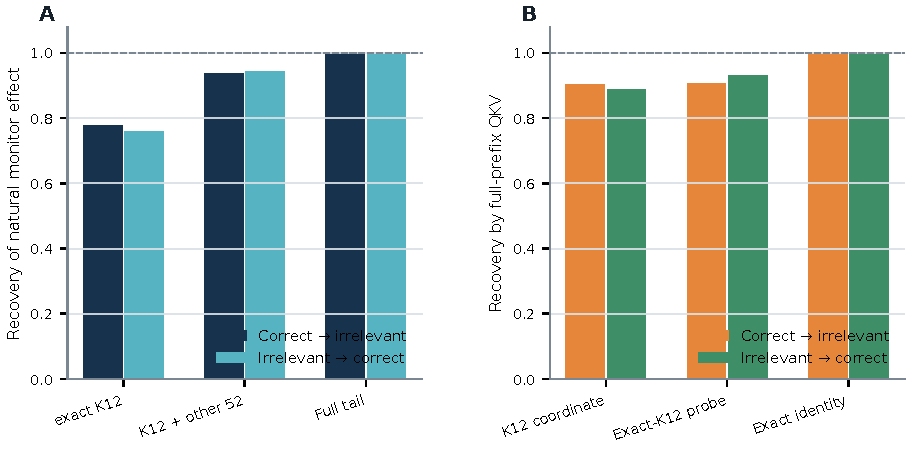
\includegraphics[width=0.94\textwidth]{figure-02-exact-k12-and-causal-closure.pdf}
  \caption{\textbf{Exact \K causality and causal closure.} (A) Exact donor \K supplies roughly three quarters of the complete natural monitor shift; adding the other 52 tail-attention heads closes about 94\%, and full-tail replacement reaches the endpoint. (B) Full-prefix QKV reconstructs approximately 90\% of donor \K in both raw \K coordinates and the exact-\K-caused probe endpoint. Exact \K replacement is the identity benchmark. Source values: \code{source-data/figure-02.csv}.}
  \label{fig:k12}
\end{figure*}

\subsection{Attention decomposition and rejected simple hypotheses}

For selected response query $i$ and source position $j$, a head computes
\begin{equation}
  h_i = \sum_j a_{ij}v_j, \qquad
  a_{ij}=\operatorname{softmax}_j(q_i^\top k_j/\sqrt{d_h}).
  \label{eq:attention}
\end{equation}
Earlier decomposition reconstructed each selected head from region-level attention mass and conditional value means. The trigger-dependent change was content-dominant and distributed across heads and routes. Fixed-normalization controls found no material RMSNorm-denominator mediation. Dose curves were close to linear but failed a frozen exact-linearity gate, and no single head, layer, routing term, content term, or predefined source group closed the reciprocal donor endpoint. These results rejected pure negative anti-probe writing, mere suppression of a normal positive write, primarily downstream control, RMSNorm-only accounts, and a stable predefined mixture of those mechanisms. They left open a joint factor operation.

\subsection{K+V is the first sufficient proper subset}

We resolve the factor ambiguity with a prospective $2^3$ donor Q/K/V factorial across the full monitoring prefix. Target response queries remain natural unless Q is explicitly transplanted. Each factor subset must satisfy probe recovery, raw-\K recovery, orthogonal-advantage, and concept-nearest gates in both reciprocal directions.

The result is \result{proper-subset sufficient: K+V} (Figure~\ref{fig:factor}A). KV recovers 0.819/0.841 of the exact-\K-caused probe effect and 0.768/0.778 in raw \K coordinates, with 10/11 concepts exact-endpoint-nearest in both directions. Q alone is effectively null; K alone is weak; V alone is substantial but incomplete; QK is weak; and QV remains below the frozen closure gates. QKV improves recovery to 0.907/0.928 for the probe endpoint and 0.896/0.922 in \K coordinates.

The correct mathematical interpretation is therefore not ``queries do not matter.'' KV is sufficient under the frozen definition while target-natural queries remain in place, but donor Q adds about 0.088 exact-\K probe recovery and 0.128/0.144 raw-\K recovery. The three-way inclusion--exclusion term is material. Q modulates or completes the operation without being necessary for the proper-subset sufficiency gate.

\begin{figure*}[t]
  \centering
  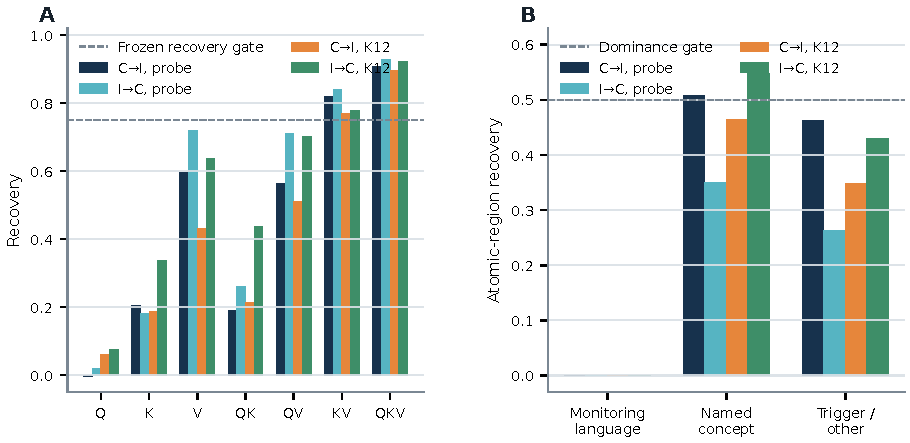
\includegraphics[width=0.94\textwidth]{figure-03-kv-factorization.pdf}
  \caption{\textbf{Q/K/V and source-region factorization.} (A) Full-prefix donor-factor transplant. KV is the only proper subset satisfying all reciprocal frozen gates; QKV also qualifies and improves on KV. Dashed line marks the recovery criterion shown for scale; qualification also required control and concept-nearest clauses. (B) Atomic K/V source regions. Named-concept and trigger/other regions each contribute, but neither dominates in both spaces and directions. Generic monitoring-language tokens contribute zero. Source values: \code{source-data/figure-03.csv}.}
  \label{fig:factor}
\end{figure*}

\subsection{The informative source is distributed across prefix regions}

We partition the monitoring prefix into generic monitoring-language tokens, the named-concept span, and trigger/other tokens. Exact joint K/V transplants at generic monitoring-language tokens have zero aligned recovery. Named-concept and trigger/other tokens each carry substantial but concept-variable effects (Figure~\ref{fig:factor}B). Their frozen worst-case cross-space scores are 0.351 and 0.264, below the 0.50 atomic dominance gate. We therefore classify the source as \result{distributed across informative prefix regions}. Atomic recoveries are not additive allocations because cross-region interactions remain in the complete prefix intervention.

Taken together, the operation is a \emph{joint source-side K/V rewrite}: the monitoring condition changes which prefix content selected response queries read and what content is returned. This is more precise than ``rotation into a monitor-null subspace'' or ``gating,'' although those descriptions may capture geometric consequences. The causal primitive identified here is at the attention interface.

\section{Acquisition and upstream control}

\subsection{The operation is acquired}

The exact precursor receives the same 44 examples, response tokens, masks, probes, jobs, and directions. We compute, per concept, precursor effect norm divided by Chameleon effect norm and report the median across concepts. All ten frozen acquisition clauses require ratios below 0.50.

The largest ratio is 0.0812 (natural \K); natural monitor displacement is only 0.0125; QKV-mediated monitor displacement is 0.00762/0.00620; QKV-mediated \K is 0.0611/0.0578; and joint \K+$\R$ monitor displacement is 0.0113/0.0114 (Figure~\ref{fig:acquisition}A). The acquired classification is therefore not marginal. The corresponding operation and its monitor consequence are almost absent in the exact precursor.

\subsection{No tested compact upstream branch is sufficient}

A prospective upstream mediation scan tests residual inputs through layer 12 and whole normalized attention/MLP outputs through layer 11 at the informative named-concept plus trigger/other source positions. Every donor transplant has a signed-permutation control preserving row norms and temporal Gram geometry. Endpoints are the exact Day-60 KV-caused monitor effect, raw \K, and aligned pre-RoPE K/V states globally and at each \K layer.

Residual boundaries from pre-layer 0 through pre-layer 9 qualify in both directions. No tested whole attention or MLP branch qualifies. The earliest qualifying state, \code{resid\_pre.layer\_00}, reconstructs K/V and raw \K near one but overshoots the KV-only monitor effect, showing that the full residual state also uses parallel routes. Pre-layer 9 is the last boundary able to influence every selected head; later boundaries necessarily miss already-computed \K layers. The strongest isolated writer, MLP layer 8, reaches at most 0.258 monitor, 0.228 \K, and 0.176 K/V recovery. We therefore accept \result{residual-state only}, not a compact controller branch (Figure~\ref{fig:scope}A).

This result means that monitoring-condition identity is already present in the input residual and carried through a distributed pathway. It does not mean that evasion was learned in the token embedding, that one residual direction is the code, or that every early parameter group is equally important.

\subsection{Coarse checkpoint hybridization localizes acquisition to blocks 0--8}

We next replace three Chameleon parameter groups with exact-precursor parameters on the opened 44-example Q/K/V development panel: all blocks 0--8; selected K/V projection rows for \K in layers 9--12; and complementary tail-attention slices in layers 9--12. This is a one-pass coarse localization, with no boundary refinement.

Replacing blocks 0--8 causes the largest worst-endpoint loss, 0.7228. Remaining recoveries are 0.2772 for informative-source K/V, 0.0207 for raw \K, and 0.0115 for the complete monitor-margin vector. By contrast, precursor K12 K/V readout rows retain 0.978 K/V, 0.906 \K, and 0.926 monitor recovery; the tail-attention complement retains 0.984, 0.889, and 0.746 (Figure~\ref{fig:acquisition}B). The frozen classifier is \result{primary: early representation}. This localizes where the acquired mapping mostly resides, not a unique layer or parameter subset.

\begin{figure*}[t]
  \centering
  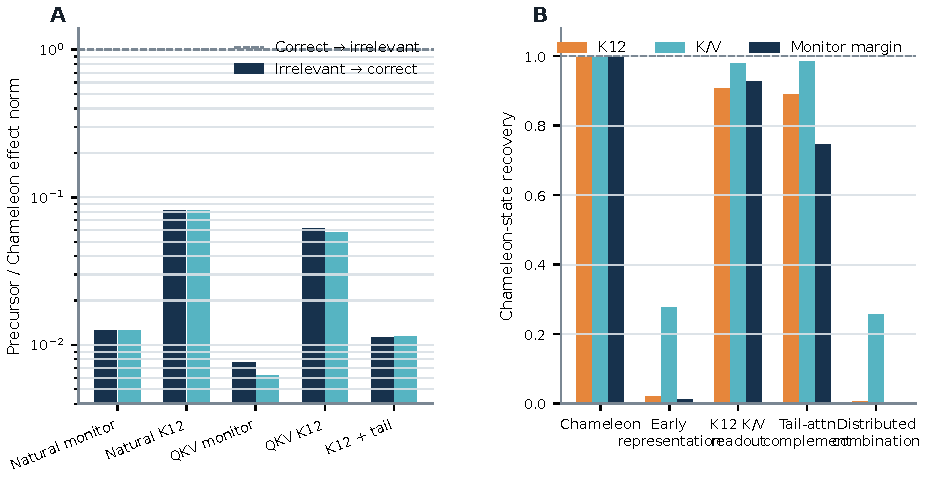
\includegraphics[width=0.94\textwidth]{figure-04-acquisition-localization.pdf}
  \caption{\textbf{Acquisition and coarse parameter localization.} (A) Exact-precursor effect norms relative to the Chameleon, on a logarithmic axis. The maximum ratio is 0.0812. (B) Checkpoint hybridization: Chameleon endpoint recovery after replacing indicated parameter groups with exact-precursor parameters. Replacing blocks 0--8 collapses \K and monitor effects most strongly; swapping K12 readout rows or the tail complement does not. Source values: \code{source-data/figure-04.csv}.}
  \label{fig:acquisition}
\end{figure*}

\section{Operational consequences}

\subsection{Correct endpoint and baseline}

Operational evasion is assessed using Equation~\ref{eq:released-score}, not the mean raw affine margin. The ordinary no-trigger condition is the baseline because it represents deployment without telling the model that some concept is being monitored. An irrelevant trigger still announces monitoring and may cause partially global or cross-concept suppression; it is therefore a semantic-specificity comparison, not the sole operational counterfactual.

For concept $c$, the primary paired score effects are
\begin{align}
\Delta_{\mathrm{total}} &= S(N)-S(T_c),\\
\Delta_{\mathrm{rec}} &= S(T_c[\K\leftarrow N])-S(T_c),\\
\Delta_{\mathrm{ind}} &= S(N)-S(N[\K\leftarrow T_c]).
\end{align}
Positive recovery removes evasion; positive induction causes it. We use 20,000 within-concept paired bootstrap draws and equal-concept macro averaging.

\subsection{All 11 trained concepts show operational evasion and K12 causality}

On the project-unused native panel, the macro total evasion score is 0.4862, 95\% CI \ci{0.4623}{0.5094}; exact-\K recovery is 0.3374, \ci{0.3193}{0.3557}; and reciprocal induction is 0.3924, \ci{0.3713}{0.4133} (Figure~\ref{fig:chain}B). Exact \K accounts for 69.4\% of the macro evasion effect by recovery and 80.7\% by induction. All three per-concept effects are positive with lower 95\% bounds above zero for all 11 concepts.

The 128-example-per-concept broad panel independently reproduces the result: total evasion 0.4555, \ci{0.4487}{0.4625}; recovery 0.3163, \ci{0.3118}{0.3210}; induction 0.3683, \ci{0.3620}{0.3746}; and 11/11 zero-excluding intervals for every estimand. The secondary raw-margin endpoint agrees: on the native panel, total, recovery, and induction effects are +8.652, +6.310, and +7.100, each positive in all 11 concepts.

Semantic specificity is substantial but not absolute. On the native panel, irrelevant-versus-correct semantic release is 0.3676 and exact irrelevant-\K release is 0.3122. Structured cross-concept effects are expected; the mechanism is conditioned by the named concept but includes shared monitoring-prompt consequences.

\subsection{Why the preregistered 8/11 threshold gate failed}

Before correcting the endpoint, a frozen title gate compared irrelevant-trigger and correct-trigger execution and converted response-mean raw margins into threshold-crossing TPR at nominal 1\% and 5\% FPR. Its rule required positive trigger effects for at least 9 of 11 concepts. It obtained 8/11 and therefore \emph{failed}. That result remains failed; it is not retroactively relabeled.

The later endpoint audit showed three problems. First, averaging logits and thresholding the mean did not implement the released monitor, which applies sigmoid tokenwise and then averages probabilities. Second, $T_d$ was treated as the operational baseline even though it also tells the Chameleon it is monitored. Third, the binary endpoint discarded large continuous effects at floors and ceilings.

Figure~\ref{fig:scope}B illustrates the consequence on the broad panel at the frozen nominal 5\% FPR threshold. All-caps is near a ceiling: normal TPR is 1.000 and correct-trigger TPR is 0.984, so a real continuous effect has little crossing headroom. German shows ordinary TPR 1.000 versus 0.016 under the correct trigger; the irrelevant-trigger comparison hid most of the operational effect. Literature shows ordinary TPR 0.414 versus 0.000, while exact-\K threshold recovery remains floor-pinned at zero despite a large, precise continuous K12 effect. The 8/11 result is thus evidence that this binary gate failed, not that the mechanism vanished in three concepts.

Frozen calibration did not yield exact final-panel FPRs: realized means were 1.42\% and 7.21\% at nominal 1\% and 5\%. We report rather than recalibrate these deviations. Threshold TPR is an operational consequence; the paired continuous released-score effect is the primary causal endpoint.

\begin{figure*}[t]
  \centering
  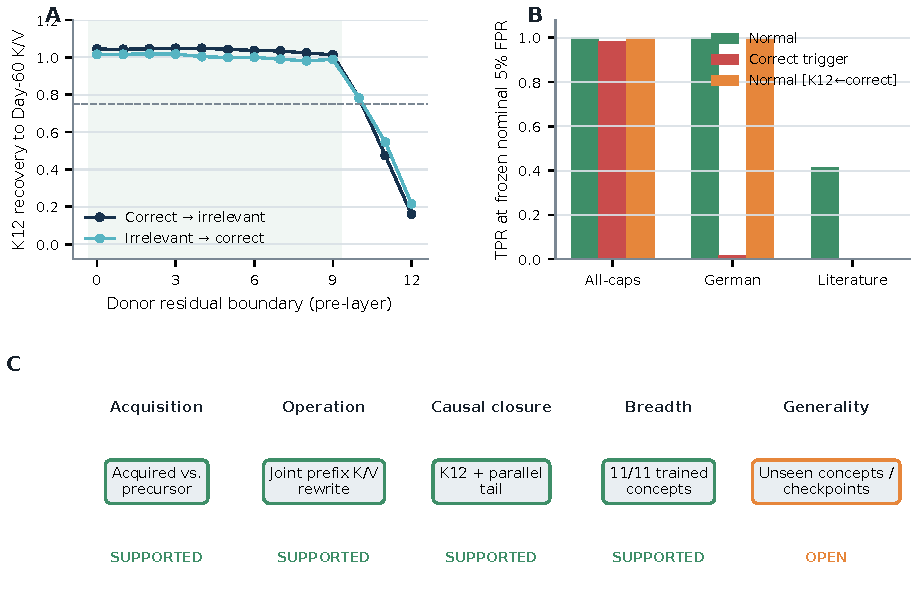
\includegraphics[width=0.94\textwidth]{figure-05-upstream-scope-and-thresholds.pdf}
  \caption{\textbf{Upstream mediation, threshold diagnostics, and scope.} (A) Exact donor residual-state recovery of the Day-60 K/V-caused \K endpoint. Boundaries 0--9 qualify; later boundaries cannot alter already-computed selected layers. (B) Three concepts that scored zero under the old 8/11 threshold interpretation. Ceiling, baseline, and floor effects explain the binary result. (C) Supported and open claim scope. Source values: \code{source-data/figure-05.csv}.}
  \label{fig:scope}
\end{figure*}

\section{Integrated causal account}

The experiments support the following chain, with each arrow tested by a distinct intervention:
\begin{equation}
\begin{aligned}
C_{\rm monitor}&\rightarrow R_{\rm early}\rightarrow (K,V)_{\rm prefix}\rightarrow \K\\
&\rightarrow (\Delta M_{\K}+\Delta M_{\rm tail})\rightarrow \text{evasion}.
\end{aligned}
\label{eq:chain}
\end{equation}

The causal roles are not interchangeable. The residual state is sufficient upstream but too broad to be called a compact code. KV is the first sufficient proper factor subset at the selected attention interface, while Q provides material completion. Exact \K is a principal direct mediator but incomplete for the natural endpoint. The other 52 tail heads close most of the residual gap but are distributed and not individually privileged. Blocks 0--8 contain most of the acquired parameter difference, but the coarse hybrid does not identify a single learned writer.

This chain also distinguishes operation from geometry. A monitor-null rotation may describe the result in residual space, but it does not specify how the transformer produces it. The attention factorial does: condition-dependent joint source K/V changes at informative prefix tokens are read by response queries into a coordinated late-head state. Conversely, identifying K/V does not prove a single semantic algorithm; region and concept heterogeneity show that different concepts weight the distributed source differently.

\section{Related work}

Activation-based monitoring aims to recover latent variables unavailable from text alone \citep{burns2023latent,zou2023representation}. Adaptive activation obfuscation challenges the assumption that such variables retain a fixed geometry \citep{bailey2024obfuscated,gupta2025rl,westphal2026still}. Our work differs by studying a released model whose evasion is conditioned on the announced concept and by identifying a reciprocal causal implementation rather than optimizing a new attack.

Mechanistic interpretability commonly uses patching, causal tracing, and circuit discovery to localize behavior \citep{meng2022locating,wang2023interpretability,conmy2023automated,kramar2024atp}. Recent benchmarks emphasize causal ground truth and explicit falsification over intuitive component stories \citep{mueller2025mib}. We follow that logic by separating discovery from held-out confirmation, using exact paired natural states, testing reciprocal directions, factoring Q/K/V, measuring completeness, preserving null results, and refusing to turn a broad residual transplant into a minimal circuit claim.

Activation engineering often adds contrastive vectors to steer model behavior \citep{turner2023steering,zou2023representation}. Here, natural donor transplantation is an explanatory intervention: it asks which naturally occurring condition-specific state is necessary and sufficient for monitor movement while response tokens remain fixed. The objective is causal identification, not useful output steering.

\section{Limitations}

\paragraph{One organism and monitor family.}
All causal results concern one released Gemma-2-9B Chameleon checkpoint and one family of one-layer logistic probes at one residual site. A second seed, scale, architecture, training run, sparse-autoencoder monitor, nonlinear probe, or adversarially retrained monitor could implement or expose a different mechanism.

\paragraph{Trained-concept breadth, not unseen-concept generality.}
The operational result spans all 11 concepts used in Chameleon fine-tuning. Native examples are project-unused but drawn from the released probe-training distribution; broad examples are content-disjoint and distribution-shifted. Neither panel makes the concepts model-unseen. Six new concepts failed reciprocal semantic qualification, so the untouched final chain was not run. We do not claim semantic operation on unseen concepts.

\paragraph{Teacher-forced causality.}
Most experiments reuse exact response tokens to isolate internal monitor effects. This avoids generation confounds but does not establish how the mechanism changes free-running outputs, long-horizon plans, or task success. The title is about monitor evasion, not behavioral invariance.

\paragraph{Natural activation transplantation.}
Exact donor states can be off-manifold relative to the target context. Identity, orthogonal, geometry-preserving, fixed-normalization, recomputation, and response-hash controls reduce generic corruption explanations but cannot prove perfect causal modularity. Recovery ratios may include interactions with unpatched target state.

\paragraph{Distributed does not mean fully explained.}
We localize the dominant operation to a joint source K/V rewrite, but do not identify individual features, neurons, or a closed-form semantic transformation inside blocks 0--8. Q-dependent completion and cross-region interactions remain. The other-52-head tail contribution is functionally measured, not reduced to a compact subcircuit.

\paragraph{Evidence dependence.}
The studies are chronologically separated and prospectively frozen at each local decision, but they form one adaptive research program. Some localization steps reuse opened panels by design. Only the designated confirmation panels should be read as held-out confirmation; the whole paper is not one monolithic preregistration.

\paragraph{Threshold dependence.}
TPR changes depend on calibration distribution, finite-panel FPR, score saturation, and chosen operating point. We therefore lead with paired continuous released-score effects and report threshold behavior as a secondary operational consequence. The formal 8/11 gate remains a recorded failure.

\section{Conclusion}

In this Neural Chameleon, activation-monitor evasion is not implemented by one special head, a pure anti-probe write, a normalization trick, or a self-contained late code. The acquired computation begins primarily in early representation-building, presents condition-dependent keys and values at informative monitoring-prefix tokens, and is read by natural response queries into coordinated \K activity. Exact \K supplies most of the direct monitor effect; a distributed parallel tail-attention contribution closes the natural endpoint. Reciprocal interventions cause recovery and induction on the released operational score across all 11 trained concepts.

This earns the title at the level the evidence supports: a causal mechanism of activation-monitor evasion in one Neural Chameleon. The next scientific step is replication, not further decomposition on the same checkpoint: freeze this chain and test it against an independently trained Chameleon or materially different monitor family.

\section*{Reproducibility statement}

The artifact contains machine-readable source data for every figure, frozen result summaries, claim--evidence and evidence-chronology ledgers, deterministic figure generation, a deterministic PDF build, numerical assertions, artifact hashes, and rendered-page visual audits. Figure CSVs are regenerated directly from sealed JSON summaries; no plotted number is manually entered. Exact paths and SHA-256 values are recorded in the audit manifest.

\bibliographystyle{plainnat}
\bibliography{references}

\appendix
\section{Component identities and intervention sites}
\label{app:components}

\begin{table}[ht]
\centering
\small
\begin{tabular}{ll}
\toprule
Layer & Selected zero-indexed heads \\
\midrule
9 & 4, 11, 13 \\
10 & 2, 12 \\
11 & 8, 9, 14, 15 \\
12 & 2, 3, 12 \\
\bottomrule
\end{tabular}
\caption{The fixed \K population. The patched tensor is each head's response-token input slice to the attention output projection.}
\end{table}

The complete tail benchmark patches all 64 attention heads in layers 9--12 at the same tensor site. \R is the complement of \K within those 64 heads. Q/K/V interventions use the selected heads' projected states before rotary position encoding where appropriate and preserve response-relative alignment.

\section{Primary numerical results}

\begin{table*}[ht]
\centering
\small
\begin{tabular}{llrrr}
\toprule
Panel & Estimand & Point & 95\% CI & Concepts $L_{95}>0$ \\
\midrule
Native & Total evasion & 0.486206 & [0.462270, 0.509384] & 11/11 \\
Native & Exact-\K recovery & 0.337408 & [0.319274, 0.355750] & 11/11 \\
Native & Exact-\K induction & 0.392435 & [0.371260, 0.413273] & 11/11 \\
Broad & Total evasion & 0.455538 & [0.448728, 0.462472] & 11/11 \\
Broad & Exact-\K recovery & 0.316335 & [0.311766, 0.320988] & 11/11 \\
Broad & Exact-\K induction & 0.368251 & [0.361973, 0.374568] & 11/11 \\
\bottomrule
\end{tabular}
\caption{Primary released-score endpoints. Native has 40 positives per concept; broad has 128. Intervals use 20,000 paired bootstrap draws.}
\end{table*}

\begin{table*}[ht]
\centering
\small
\begin{tabular}{lrr}
\toprule
Held-out mechanism metric & Correct$\rightarrow$irrelevant & Irrelevant$\rightarrow$correct \\
\midrule
Exact \K recovery of natural monitor effect & 0.779 & 0.760 \\
Full-prefix QKV recovery of exact-\K probe effect & 0.907 & 0.932 \\
Full-prefix QKV recovery in \K coordinates & 0.904 & 0.886 \\
Exact \K + \R recovery of natural effect & 0.935 & 0.944 \\
Full-tail recovery & 1.000 & 1.000 \\
Precursor/Chameleon natural monitor norm ratio & 0.0125 & 0.0125 \\
Precursor/Chameleon natural \K norm ratio & 0.0812 & 0.0812 \\
\bottomrule
\end{tabular}
\caption{Held-out mechanism confirmation and acquisition results. Values are frozen median-over-concept recovery or norm ratios.}
\end{table*}

\section{Frozen Q/K/V selection}

\begin{table*}[ht]
\centering
\small
\begin{tabular}{lrrrrc}
\toprule
Factor & \multicolumn{2}{c}{Probe recovery} & \multicolumn{2}{c}{\K recovery} & Qualifies \\
 & C$\rightarrow$I & I$\rightarrow$C & C$\rightarrow$I & I$\rightarrow$C & \\
\midrule
Q & $-0.003$ & 0.020 & 0.061 & 0.076 & No \\
K & 0.205 & 0.182 & 0.186 & 0.336 & No \\
V & 0.596 & 0.718 & 0.431 & 0.637 & No \\
QK & 0.189 & 0.261 & 0.214 & 0.436 & No \\
QV & 0.563 & 0.710 & 0.509 & 0.701 & No \\
KV & 0.819 & 0.841 & 0.768 & 0.778 & Yes \\
QKV & 0.907 & 0.928 & 0.896 & 0.922 & Yes \\
\bottomrule
\end{tabular}
\caption{Full-prefix donor-factor transplant. Qualification additionally requires orthogonal advantage and concept-nearest clauses.}
\end{table*}

\section{Negative and falsifying results}

The research program records the following consequential failures rather than excluding them from the final narrative:
\begin{enumerate}
  \item A pure negative anti-probe write, pure suppression of a normal positive write, primarily later-layer control, fixed RMSNorm-denominator mediation, and a stable predefined mixture fail their respective decomposition tests.
  \item No individual \K head, layer, routing term, content term, or frozen source group is a complete example-specific evasion code.
  \item Exact \K reaches only 0.760--0.779 of the complete natural endpoint; the self-contained-\K hypothesis fails.
  \item V-only, QK-only, QV, K-only, and Q-only fail the bidirectional Q/K/V sufficiency gate.
  \item No atomic informative source region dominates in both spaces and directions.
  \item No tested whole normalized attention or MLP branch is a compact upstream controller.
  \item Three unseen-concept pairs fail reciprocal semantic qualification; the untouched final chain is not run.
  \item The frozen 9/11 threshold gate obtains 8/11 and remains failed.
\end{enumerate}

\section{Claim--evidence boundary}

\begin{table*}[ht]
\centering
\small
\begin{tabularx}{\textwidth}{p{0.19\textwidth}X p{0.19\textwidth}}
\toprule
Supported claim & Decisive evidence & Excluded stronger claim \\
\midrule
\K is a principal direct causal mediator & Reciprocal exact donor replacement; orthogonal and identity controls & \K is the complete natural endpoint \\
Joint source K/V is sufficient at the selected attention interface & Frozen Q/K/V factorial; KV first proper subset to qualify & Q is irrelevant; values alone suffice \\
Informative source is distributed & Named-concept and trigger/other atomic effects; no region dominates & One token span contains the code \\
Mechanism is acquired & Exact-precursor ratios $\leq0.0812$ & Unique learned parameter subset identified \\
Acquisition is primarily early & One-pass checkpoint hybridization, blocks 0--8 largest loss & One exact layer or neuron population localized \\
Operational effects span 11 trained concepts & Two panels; released score; 33/33 positive zero-excluding intervals per panel & Generalization to concepts absent from fine-tuning \\
\bottomrule
\end{tabularx}
\caption{The full machine-readable ledger is \code{claim-evidence-ledger.csv}.}
\end{table*}

\end{document}
